\vspace{-1cm}
\begin{figure}
	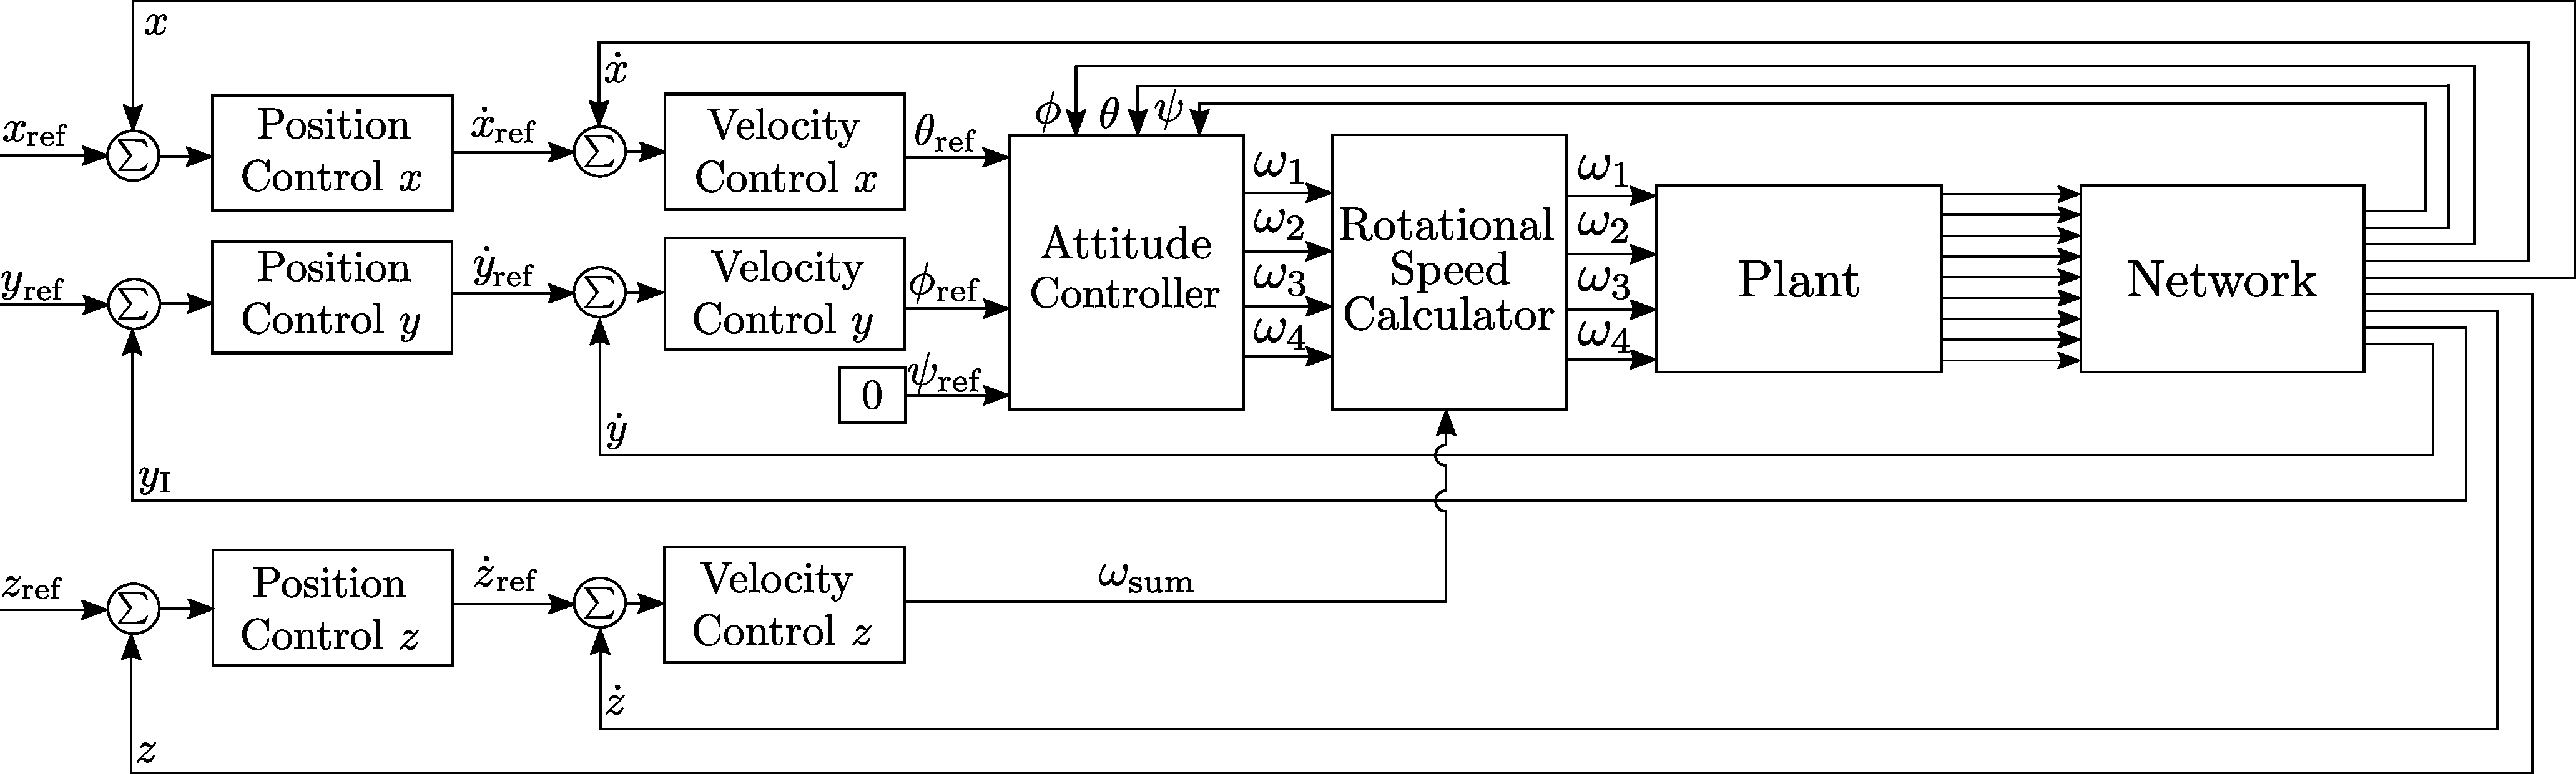
\includegraphics[width=0.7\linewidth]{figures/TranslationalControlDiagram}
	\caption{Figure caption}
\end{figure}

\begin{columns}[t,totalwidth=\twocolwid] % Split up the two columns wide column

	\begin{column}{0.49\twocolwid} % The first column within column 2 (column 2.1)
  	 \centering
  	 \hspace{-2cm}
  	 \parbox{.88\textwidth}{
    	 \begin{itemize}
  	 			\item[]\textbf{Attitude controller}\\
  	 			\item State feedback with integral controller designed with LQR is used for tracking references and handling disturbances.
  	 			\item A reduced order observer is used to estimate the angular velocities.
  	 			\item[]\vspace{5pt}
  	 			%\vspace{39pt}
  	 			%\vspace{5pt}
  	 			%State feedback with integral control, to be able to track references and handle disturbances, is used along with a reduced order observer, estimating angular velocities.
  	 		\end{itemize}
  	 }
	\end{column} % End of column 2.1
	\hspace{-4cm}
	\begin{column}{0.5\twocolwid} % The second column within column 2 (column 2.2)
  	 \centering
   	 \parbox{1\textwidth}{
       	 \begin{itemize}
    	 			\item[]\textbf{Translational controllers}\\
     	 			\item PI controllers are used to control the translational velocities
     	 			\item The outer loops are P controllers used to control the translational position.
     	 			\item The bandwidth of the cascaded controllers is taken into account to reduce the effect of the dynamics of the inner loop in the outer loop.
       	 \end{itemize}		
   	 }
	\end{column} % End of column 2.2
	\vspace{-.5cm}
\end{columns} % End of the split of column 2 - any content after this will now take up 2 columns width